%%%
% Plantilla de Memoria
% Modificación de una plantilla de Latex de Nicolas Diaz para adaptarla 
% al castellano y a las necesidades de escribir informática y matemáticas.
%
% Editada por: Mario Román
%
% License:
% CC BY-NC-SA 3.0 (http://creativecommons.org/licenses/by-nc-sa/3.0/)
%%%

%%%%%%%%%%%%%%%%%%%%%%%%%%%%%%%%%%%%%%%%%
% Thin Sectioned Essay
% LaTeX Template
% Version 1.0 (3/8/13)
%
% This template has been downloaded from:
% http://www.LaTeXTemplates.com
%
% Original Author:
% Nicolas Diaz (nsdiaz@uc.cl) with extensive modifications by:
% Vel (vel@latextemplates.com)
%
% License:
% CC BY-NC-SA 3.0 (http://creativecommons.org/licenses/by-nc-sa/3.0/)
%
%%%%%%%%%%%%%%%%%%%%%%%%%%%%%%%%%%%%%%%%%

%----------------------------------------------------------------------------------------
%	PAQUETES Y CONFIGURACIÓN DEL DOCUMENTO
%----------------------------------------------------------------------------------------

%%% Configuración del papel.
% microtype: Tipografía.
% mathpazo: Usa la fuente Palatino.
\documentclass[a4paper, 20pt]{article}
\usepackage[a4paper,margin=1in]{geometry}
\usepackage[protrusion=true,expansion=true]{microtype}
\usepackage{mathpazo}

% Indentación de párrafos para Palatino
\setlength{\parindent}{0pt}
  \parskip=8pt
\linespread{1.05} % Change line spacing here, Palatino benefits from a slight increase by default


%%% Castellano.
% noquoting: Permite uso de comillas no españolas.
% lcroman: Permite la enumeración con numerales romanos en minúscula.
% fontenc: Usa la fuente completa para que pueda copiarse correctamente del pdf.
\usepackage[spanish,es-noquoting,es-lcroman,es-tabla,,es-nodecimaldot]{babel}
\usepackage[utf8]{inputenc}
\usepackage{fontenc}
\selectlanguage{spanish}


%%% Gráficos
\usepackage{graphicx} % Required for including pictures
\usepackage{wrapfig} % Allows in-line images
\usepackage[usenames,dvipsnames]{color} % Coloring code
\graphicspath{{./fig/}}


%%% Matemáticas
\usepackage{amsmath}

%%% Pseudocódigo
\usepackage{algorithmicx}
\usepackage[ruled]{algorithm}
\usepackage{algpseudocode}

\newcommand{\alg}{\texttt{algorithmicx}}
\newcommand{\old}{\texttt{algorithmic}}
\newcommand{\euk}{Euclid}
\newcommand\ASTART{\bigskip\noindent\begin{minipage}[b]{0.5\linewidth}}
\newcommand\ACONTINUE{\end{minipage}\begin{minipage}[b]{0.5\linewidth}}
\newcommand\AENDSKIP{\end{minipage}\bigskip}
\newcommand\AEND{\end{minipage}}

%%% Código
\usepackage{listings}

%%% Tablas
\usepackage{tabularx}
\usepackage{float}
\usepackage{adjustbox}
\usepackage{booktabs}

% Enlaces y colores
\usepackage{hyperref}
\usepackage[dvipsnames]{xcolor}
\definecolor{webgreen}{rgb}{0,0.5,0}
\hypersetup{
  colorlinks=true,
  citecolor=RoyalBlue,
  urlcolor=RoyalBlue,
  linkcolor=RoyalBlue
}

%%% Bibliografía
\usepackage[backend=biber]{biblatex}
\DefineBibliographyStrings{spanish}{
  urlseen = {Último acceso}
}
\addbibresource{IN-P2.bib}

%----------------------------------------------------------------------------------------
%	TÍTULO
%----------------------------------------------------------------------------------------
% Configuraciones para el título.
% El título no debe editarse aquí.
\renewcommand{\maketitle}{
  \begin{flushright} % Right align
  
  {\LARGE\@title} % Increase the font size of the title
  
  \vspace{50pt} % Some vertical space between the title and author name
  
  {\large\@author} % Author name
  \\\@date % Date
  \vspace{40pt} % Some vertical space between the author block and abstract
  \end{flushright}
}

%% Título
\title{\textbf{Título}\\ % Title
Subtítulo} % Subtitle

\author{\textsc{Autor1,\\Autor2} % Author
\\{\textit{Universidad de Granada}}} % Institution

\date{\today} % Date

%-----------------------------------------------------------------------------------------
%	DOCUMENTO
%-----------------------------------------------------------------------------------------

\begin{document}

%-----------------------------------------------------------------------------------------
%	TITLE PAGE
%-----------------------------------------------------------------------------------------

\begin{titlepage} % Suppresses displaying the page number on the title page and the subsequent page counts as page 1
	
	\raggedleft % Right align the title page
	
	\rule{1pt}{\textheight} % Vertical line
	\hspace{0.05\textwidth} % Whitespace between the vertical line and title page text
	\parbox[b]{0.8\textwidth}{ % Paragraph box for holding the title page text, adjust the width to move the title page left or right on the page
		
		{\Huge\bfseries Práctica 2:\\[0.5\baselineskip] Análisis Relacional mediante\\ \\ Segmentación}\\[2\baselineskip] % Title
		{\large\textit{Curso 2019/2020}}\\[4\baselineskip] % Subtitle or further description
		{\Large\textsc{Sofía Almeida Bruno}\\[0.5\baselineskip]sofialmeida@correo.ugr.es} % Author name, lower case for consistent small caps
		
		\vspace{0.4\textheight} % Whitespace between the title block and the publisher
		
		{\noindent Grupo IN 2\\[0.5\baselineskip] Jueves 9:30-10:30}\\[\baselineskip] % Publisher and logo
	}

\end{titlepage}

%% Resumen (Descomentar para usarlo)
%\renewcommand{\abstractname}{Resumen} % Uncomment to change the name of the abstract to something else
%\begin{abstract}
% Resumen aquí
%\end{abstract}

%% Palabras clave
%\hspace*{3,6mm}\textit{Keywords:} lorem , ipsum , dolor , sit amet , lectus % Keywords
%\vspace{30pt} % Some vertical space between the abstract and first section


%% Índice
{\parskip=2pt
  \tableofcontents
}
\pagebreak

%%% Inicio del documento
%%%%%%%%%%%%%%%%%%%%%%%%%%%%%%%%%%%%%%%%%%%%%%%%%%%%%%%%%%%%%%%%%%%
%       DESCRIPCIÓN DEL PROBLEMA
%%%%%%%%%%%%%%%%%%%%%%%%%%%%%%%%%%%%%%%%%%%%%%%%%%%%%%%%%%%%%%%%%%%
\section{Introducción}

Tras estudiar, en la práctica anterior, algoritmos de clasificación para un problema de aprendizaje supervisado, pasamos ahora a un problema de aprendizaje no supervisado. Utilizaremos diferentes algoritmos de agrupamiento o clustering para realizar un análisis relacional.

En este caso partiremos de los microdatos publicados por el Instituto Nacional de Estadística (INE) en 2018 sobre la última encuesta de fecundidad. Elegiremos tres casos de estudio diferentes, en los que seleccionaremos las variables a estudiar (en general, de tipo categórico) y las variables sobre las que aplicar clustering (no tiene interés aplicarlo sobre el resto de variables ya que podrían no ser relevantes), compararemos distintos algoritmos y analizaremos los resultados obtenidos de forma comparada.

El conjunto original dispone de 14556 respuestas a la encuesta, con 463 variables sobre identificación, datos biográficos, hogar, vivienda, padres, relaciones de pareja actual e historia, hijos, embarazo actual y anteriores,\dots

En cada caso de estudio utilizaremos y compararemos varios algoritmos de agrupamiento, centrándonos en dos de ellos para hacer un análisis más profundo y tratando de mejorar sus resultados mediante el ajuste de sus parámetros. Los algoritmos elegidos y los parámetros con los que usarlo inicialmente son los siguientes:

\begin{itemize}
\item \textbf{K-Means}. Agrupa los ejemplos en tantos grupos como se le haya indicado. Parte de unos centros iniciales, asigna a cada ejemplo el cluster correspondiente al centro más cercano, recalcula los centros y vuelve al paso anterior. Este proceso se repite hasta que no haya más cambios en los clusters. Al estar basado en centroides generará clusters convexos. Parámetro inicial: \texttt{n\_clusters = 5}.
\item \textbf{MeanShift}. Este algoritmo está basado en la densidad de las muestras. A partir de un radio fijado, determina un número de clusters y va desplazando sus centros hacia las regiones más densas. Es otro ejemplo de algoritmo basado en centroides, los clusters generados serán también convexos. Preliminarmente estima \texttt{bandwidth} por defecto.
\item \textbf{Birch}. Agrupa los objetos según se vayan recibiendo, es un algoritmo de clustering incremental. Crea un árbol con las características de los clusters guardando solo la información necesaria para poder determinarlos. Cada nodo tendrá un número de subclusters acotado por el factor de ramificación y un umbral que determina si un nuevo ejemplo está lo suficientemente cerca del cluster para pertenecer a él. Cuando llega un objeto, desciende por el árbol escogiendo en cada nodo el de características similares. Si no pertenece a ningún cluster y no se ha superado el factor de ramificación, se crea un nuevo subcluster, en caso contrario es absorbido por el cluster en cuestión. El último parámetro a fijar es el número de clusters con el que quedarnos finalmente. Inicialmente  \texttt{branching\_factor=25}, \texttt{threshold=0.25}, \texttt{n\_clusters=5}.
\item \textbf{DBSCAN}. Es un algoritmo basado en densidad que no utiliza centroides, por lo que los grupos generados pueden tener diversas formas. Utiliza dos parámetros para definir la densidad: un valor $\varepsilon$ que determina cuándo un objeto es densamente alcanzable a partir de otro, un número mínimo de objetos por los que podemos alcanzar a otro para afirmar que pertenecen al mismo cluster. Generará en ocasiones un grupo etiquetado como ``-1'' que contiene a aquellos puntos que no pueden ser agrupados. Se comienza con \texttt{eps=0.2}\footnote{Se partió de un valor inicial $\varepsilon = 0.5$,  pero al ver que no conseguía buenos resultados en los casos a estudiar se disminuyó tratando de conseguir más variedad en los grupos.}, \texttt{min\_samples=5}.
\item \textbf{Ward}. Este método se distingue de los demás en que es jerárquico, es decir, genera una jerarquía que según el nivel de corte dará distintos agrupamientos. En este caso se ha elegido un algoritmo que en cada paso va agrupando dos clusters (inicialmente cada objeto es un cluster) de forma que el agrupamiento minimice la varianza (media de la distancia al cuadrado de cada elemento al centroide). Especificaremos como parámetro en qué nivel de la jerarquía nos quedamos, en este caso, \texttt{n\_clusters=5}.
\end{itemize}

Para comparar los resultados y rendimiento de los diferentes algoritmos según distintos índices(?):
\begin{itemize}
\item \textbf{Tiempo}. Mediremos el tiempo que tarda cada algoritmo en agrupar el mismo conjunto de datos. Aunque no es el factor más importante en clustering, puede ser determinante para decantarnos por los algoritmos más rápidos entre aquellos que consigan resultados similares lo suficientemente buenos.
\item \textbf{Calinski-Harabasz}. Es una ratio entre la dispersión intracluster e intercluster para todos los clusters, donde la dispersión se mide como la suma de las distancias al cuadrado. Un valor alto indica que los grupos son densos y están bien separados.
\item \textbf{Silhouette}. Este coeficiente mide cómo de similares son los objetos de un mismo cluster comparado con los de otros clusters. Toma valores en el intervalo $[-1,1]$. Un valor cercano a 1 indica que los clusters están muy concentrados y distantes a los demás, uno cercano a 0 señala que los clusters están superpuestos y uno cercano a -1 que el agrupamiento es incorrecto.
\item \textbf{Número de clusters}. Comparando este valor observaremos si algún algoritmo no logra agrupar correctamente, por hacer demasiados clusters o, por el contrario, por no agrupar lo suficiente. En los algoritmos que sea un parámetro fijo podemos variarlo y ver cuál es el número de clusters que mejor se adapta a nuestro conjunto.
\end{itemize}

%%%%%%%%%%%%%%%%%%%%%%%%%%%%%%%%%%%%%%%%%%%%%%%%%%%%%%%%%%%%%%%%%%%
%       Caso de estudio 1 - PRIMER HIJO CON MÁS DE 30 AÑOS
%%%%%%%%%%%%%%%%%%%%%%%%%%%%%%%%%%%%%%%%%%%%%%%%%%%%%%%%%%%%%%%%%%%
\section{Caso de estudio 1 - Primer hijo con más de 30 años}
\label{sec:caso1}
% Qué se analiza y por qué (indicar nº de datos que representa el caso de estudio)
En el resumen del INE sobre esta encuesta no se realizó un análisis de agrupamiento como el desarrollado en esta práctica, como mucho se relacionaron dos variables. Tomando como inspiración el resumen \cite{resINE} del INE, que muestra algunos resultados destacados obtenidos a partir de dicha encuesta, enfocaré el primer caso de estudio al retraso en la maternidad. Para ello, calculo (a partir de los datos dados) la edad media en la que las mujeres tienen su primer hijo: a los 24 años. Así, fijo como primer caso de estudio el conjunto de \textit{mujeres que tuvieron su primer hijo con 30 años o más}. Este subconjunto está formado por 1545 objetos.

Para realizar el agrupamiento en este conjunto selecciono cuatro variables que pueden ayudarnos a distinguir la situación y preocupaciones de las mujeres con una maternidad tardía:
\begin{itemize}
\item \textbf{NHIJOSDESEO} es el número de hijos que le gustaría o hubiera gustado tener a la entrevistada.
\item \textbf{ANORELACION} indica el año en el que comenzó la relación sentimental actual.
\item \textbf{ANOTRABACT} representa el año en el que la mujer comenzó a trabajar en su puesto actual.
\item \textbf{EDADIDEAL} como su nombre indica, es la edad que la entrevistada considera oportuna para tener el primer hijo.
\end{itemize}

Una vez fijado el caso de estudio y las variables mediante las que agrupar, utilizamos el \textit{script} \texttt{caso1.py} para ejecutar los cinco algoritmos y obtener tanto la tabla de resultados como los diferentes tipos de gráficos asociados. Podemos observar en la Tabla \ref{tab:algorithms1} los índices obtenidos en este caso de estudio.

% Tabla comparativa algotimos de clustering
\begin{table}[H]
\centering
\caption{Resultados caso de estudio 1}
\label{tab:algorithms1}
\begin{tabular}{lrrrr}
\toprule
Algoritmo & Tiempo ($s$) & Calinski-Harabasz & Silhouette & Número de clusters\\
\midrule
KMeans & 0.063 & 580.785 & 0.27533 & 5 \\
MeanShift & 9.857 & 9.770 & 0.32542 & 2 \\
Birch & 0.087 & 321.158 & 0.26552 & 5 \\
DBSCAN & 0.035 & 28.496 & 0.38585 & 2 \\
Ward & 0.099 & 501.202 & 0.29108 & 5 \\
\bottomrule
\end{tabular}
\end{table}

En una primera lectura detectamos que el tiempo de ejecución del algoritmo MeanShift es considerablemente mayor que el del resto de algoritmos. Esto se debe a que cuando lo ejecutamos, como no especificamos el valor de los parámetros, los calcula usando \texttt{sklearn.cluster.estimate\_bandwidth} que, como indica su documentación \cite{bandwidth}, tarda un tiempo cuadrático sobre el número de objetos. El tiempo de ejecución del resto de algoritmos es similar, siendo un poco menor el de KMeans y DBSCAN.

También destaca el bajo número de clusters generados por los algoritmos DBSCAN y MeanShift: 2. Esto quiere decir que formaron un único grupo (DBSCAN con el 98.83\% de los objetos, MeanShift con el 99.68\%) y juntó en el otro cluster, los objetos que no encajaban en él. Esto provoca que los objetos del cluster único estén muy separados de los del otro cluster, esta es la posible causa de que el índice Silhouette sea más elevado que en el resto de casos.

Para realizar un análisis de los grupos me centraré en los algoritmos KMeans y Birch.

\subsection{Análisis KMeans}

El algoritmo KMeans genera 5 grupos, como habíamos indicado, vemos en la Figura \ref{fig:KMeans_tam1} la distribución de los objetos en los distintos grupos.

\begin{figure}[H]
    \centering
    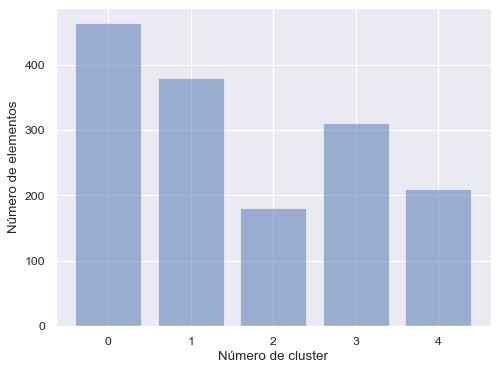
\includegraphics[width=0.6\textwidth]{./caso1/KMeans_tam_clusters}
    \caption{Caso 1 - Tamaño de los clusters- KMeans}
    \label{fig:KMeans_tam1}
\end{figure}

Los grupos tienen tamaños en rangos similares, entre 300 y 450 los tres mayoritarios, seguidos por un cluster con 209 elementos y el menor con 180. Para analizar los grupos, observamos en la Figura \ref{fig:KMeans_scatter1} la matriz de dispersión de las variables dos a dos y el histograma de cada una de ellas en la diagonal.

\begin{figure}[H]
    \centering
    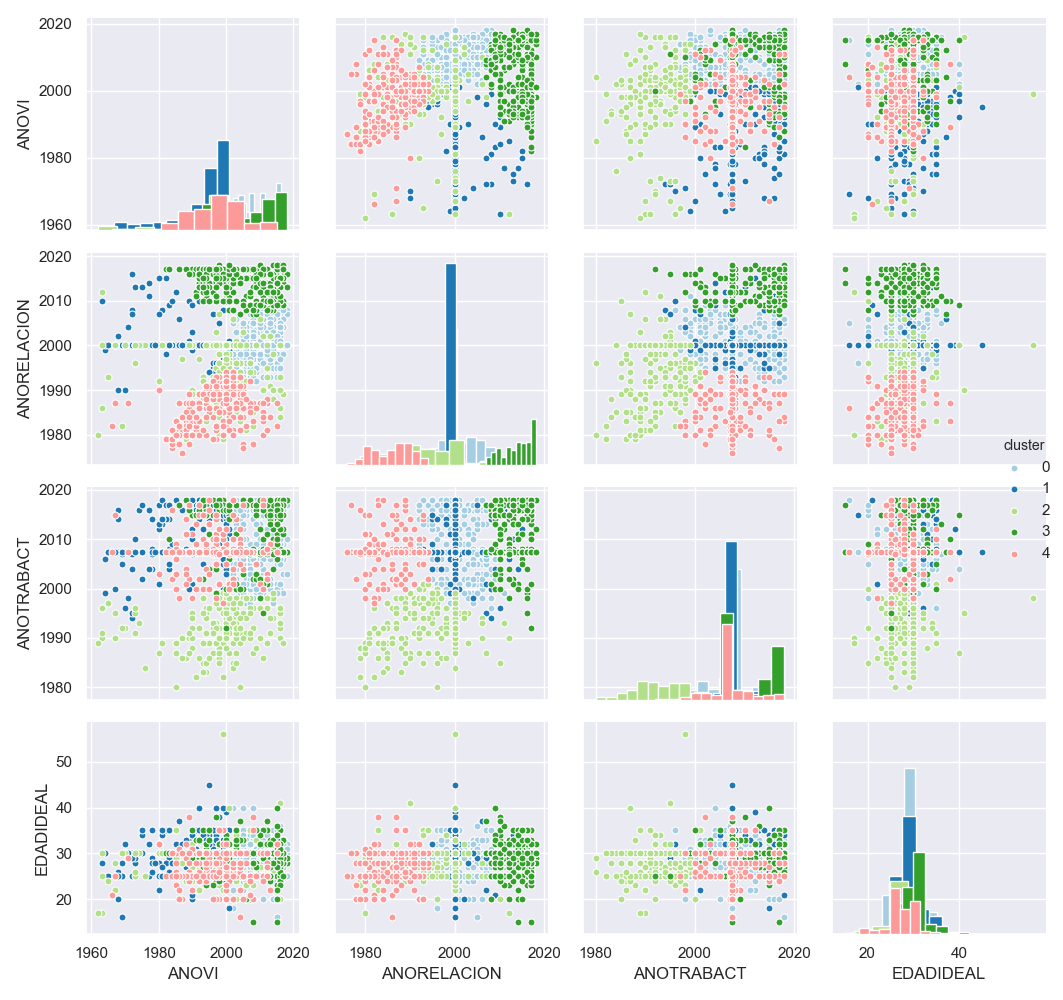
\includegraphics[width=1\textwidth]{./caso1/KMeans_scattermatrix}
    \caption{Caso 1 - Matriz de dispersión - KMeans}
    \label{fig:KMeans_scatter1}
\end{figure}

Las variables ANORELACION y ANOTRABACT sirven para separar bastante bien cuatro de los grupos, pero el resto también aporta información relevante. Aparentemente tenemos 4 grupos bien definidos y uno un poco más disperso, el cluster 1. Al cambiar el valor del parámetro \texttt{n\_clusters} descubriremos si al reagrupar se consiguen clusters más compactos. Rellenaremos la Tabla \ref{tab:carac_kmeans_1} con ayuda del diagrama de cajas mostrado en la Figura \ref{fig:KMeans_boxplot1} para hacernos una idea de las características principales de cada grupo.

\begin{figure}[H]
    \centering
    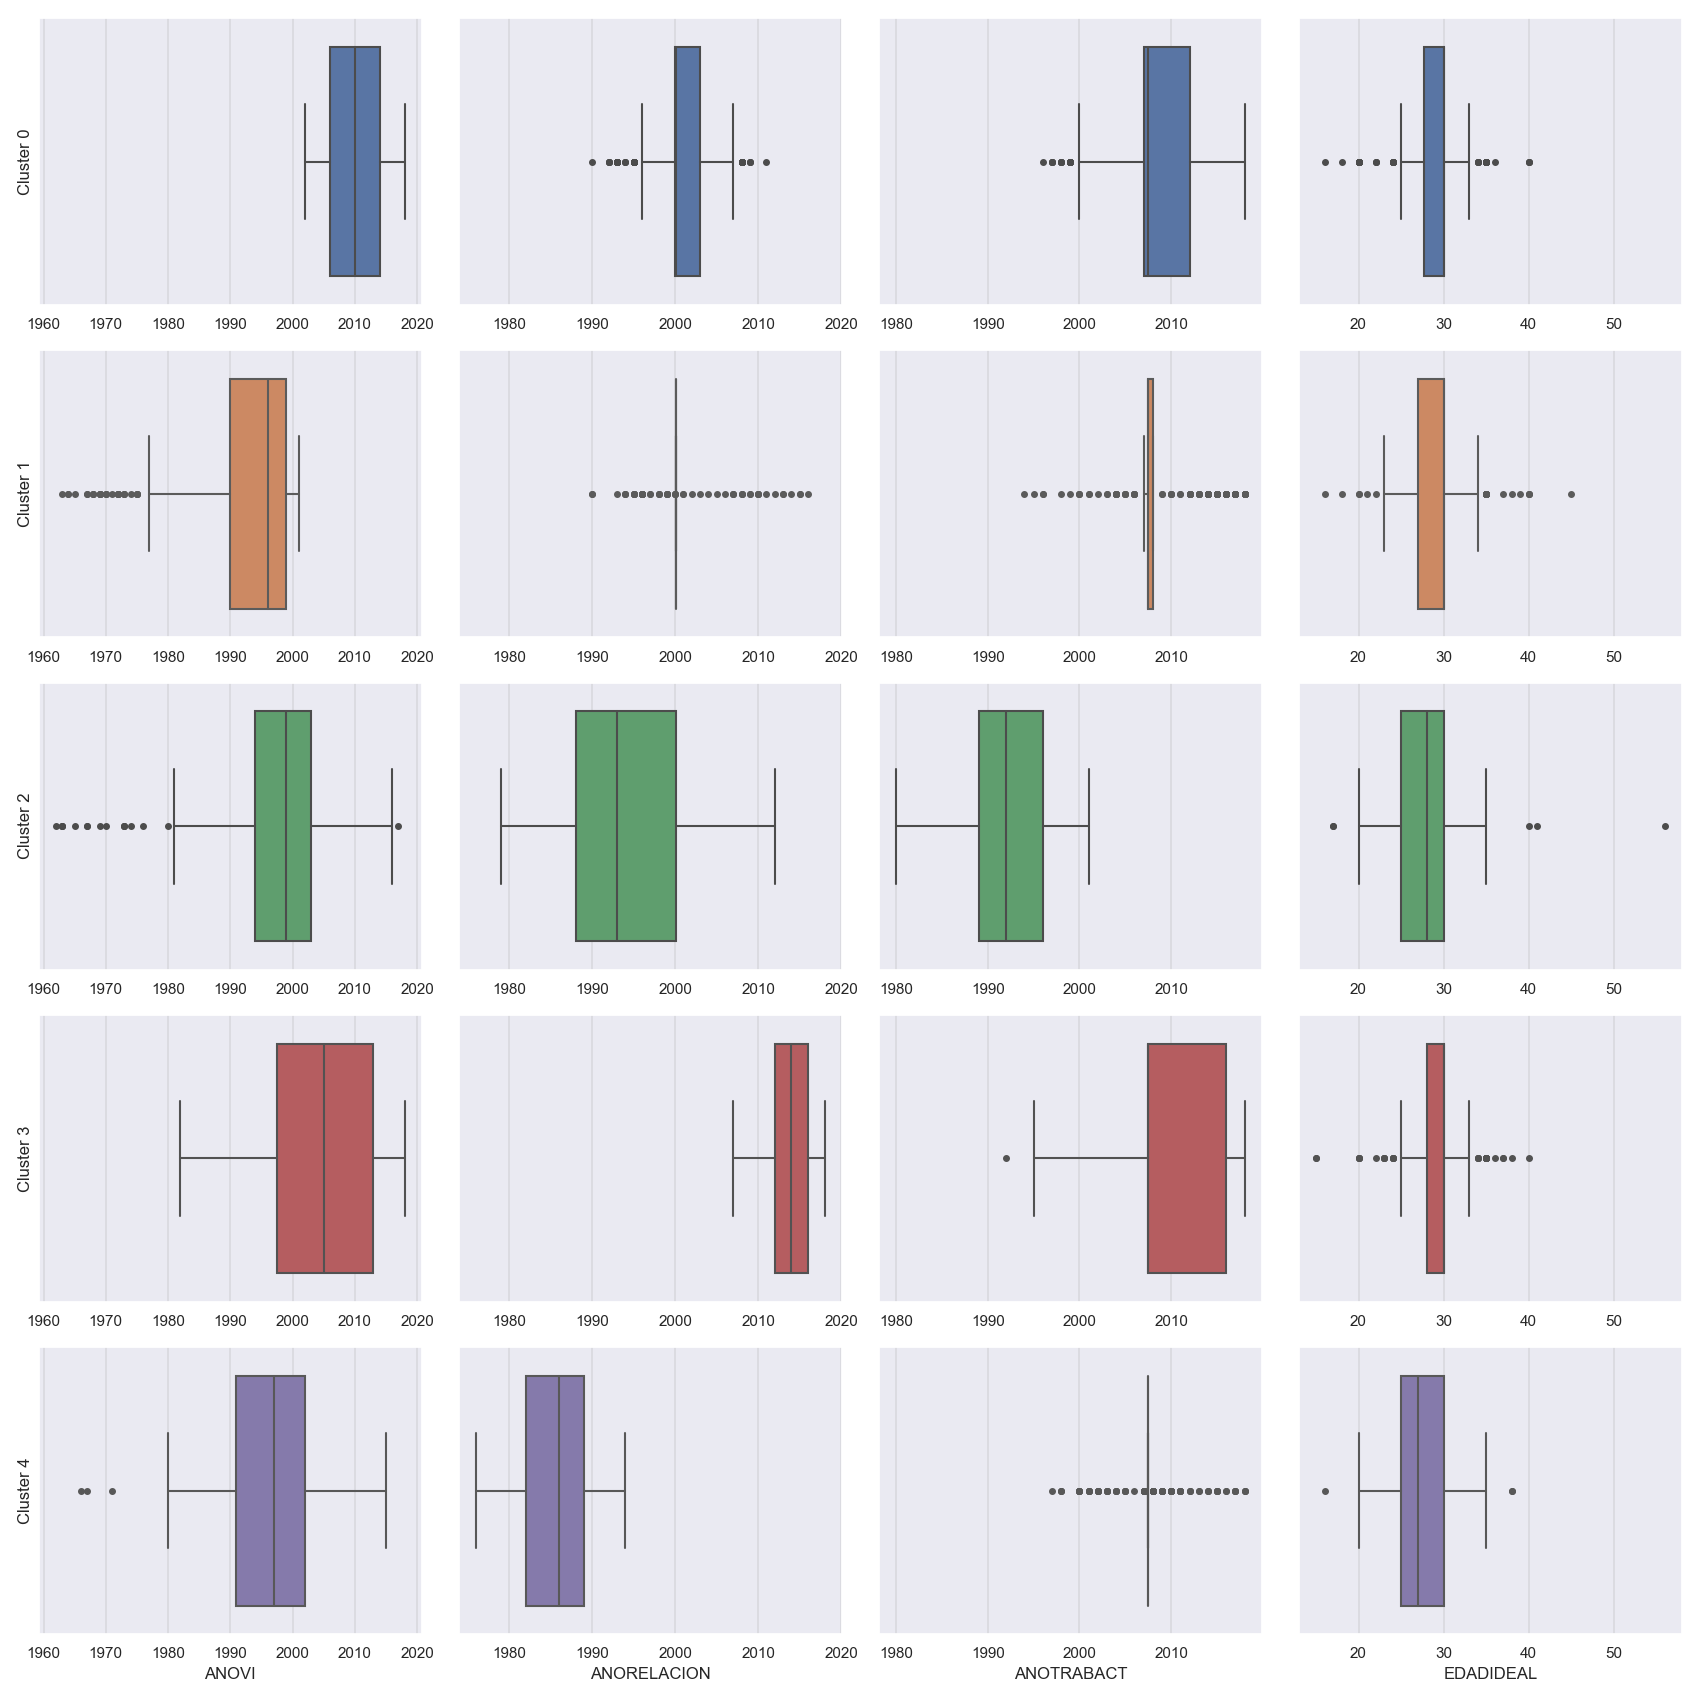
\includegraphics[width=1\textwidth]{./caso1/KMeans_boxplot}
    \caption{Caso 1 - Diagrama de cajas - KMeans}
    \label{fig:KMeans_boxplot1}
\end{figure}

% Tabla características de los grupos generados por KMeans
\begin{table}[H]
\centering
\caption{Caso 1 - Características de los grupos - KMeans}
\label{tab:carac_kmeans_1}
\begin{tabular}{lrrrr}
\toprule
Cluster & ANOVI & ANORELACION & ANOTRABACT & EDADIDEAL\\
\midrule
0 & 2005-2015 & 2000-2003 & 2007-2012 & 28-30 \\
1 & 1990-1999 & 2000 & 2008 & 27-30 \\
2 & 1995-2003 & 1987-2000 & 1988-1996 & 25-30 \\
3 & 1997-2012 & 2012-2016 & 2007-2016 & 28-30 \\
4 & 1991-2002 & 1983-1989 & 2008 & 25-30 \\
\bottomrule
\end{tabular}
\end{table}

Destaca que la mayor parte de las entrevistadas consideran que la edad ideal para tener un hijo es como mucho 30 años. Aunque en cada grupo el rango de edad que se considera apropiado para tener un hijo varía, considerando el mayor subconjunto, en general podemos afirmar que las mujeres que tuvieron el primer hijo con más de 30 años consideran que lo ideal habría sido tenerlo antes.

El cluster 0, mayoritario, está caracterizado por las mujeres que comenzaron su relación en torno al año 2000 y pasaron a vivir con su pareja a partir del año 2005. Al igual que las mujeres del cluster 3, comenzaron a trabajar en el puesto actual a partir del año 2007, posiblemente después de tener ese primer hijo. El cluster 3 es opuesto a este, está formado por aquellas mujeres que llevaban un tiempo viviendo con su pareja actual (comenzaron dicha convivencia en un rango que va desde 1997 hasta 2012) y empezaron la relación sentimental posteriormente.

La variable que más nos ayuda a distinguir el cluster 2 es ANOTRABACT, las mujeres de este grupo llevan trabajando desde el siglo anterior en el mismo empleo. Mientras que para diferenciar al cluster 4 es el año de comienzo de la relación el que nos dará la clave. Las mujeres de este cluster comenzaron su relación actual en la década de los 80.

El cluster 1, como ya habíamos observado en la matriz de dispersión, es un cluster más disperso, contiene \textit{outliers}, o valores anómalos, en todas las variables.

\subsubsection{Análisis de parámetros}

En este algoritmo el parámetro decisivo es el número de clusters. A priori, dado un conjunto de datos tan grande y sin conocimiento experto sobre el problema, es difícil acertar con el número de grupos en los que dividir el subconjunto. Podríamos aumentar este número enormemente para conseguir clusters muy compactos, el límite sería que cada objeto fuera su propio cluster, pero entonces no cumpliríamos los objetivos buscados: obtener información de los datos al agruparlos según una serie de variables.

Para probar con distintas opciones de este parámetro implementamos el \textit{script} \texttt{caso1-kmeans}, donde se ejecuta el algoritmo KMeans variando el parámetro \texttt{n\_clusters} en el rango de enteros $[2,15]$. En la Tabla \ref{tab:param_kmeans1} vemos los resultados obtenidos para cada valor del parámetro.

% Tablas comparativas para el análisis de parámetros
\begin{table}[H]
\centering
\caption{Resultados cambio de parámetros KMeans}
\label{tab:param_kmeans1}
\begin{tabular}{lrrrr}
\toprule
Número de clusters & Tiempo ($s$) & Calinski-Harabasz & Silhouette &\\
\midrule
2 & 0.023 & 680.214 & 0.32456 \\
3 & 0.024 & 580.263 & 0.26207 \\
4 & 0.038 & 560.781 & 0.24693 \\
5 & 0.052 & 587.885 & 0.31232 \\
6 & 0.064 & 588.794 & 0.28092 \\
7 & 0.079 & 583.712 & 0.29898 \\
8 & 0.128 & 578.210 & 0.30893 \\
9 & 0.159 & 559.847 & 0.30801 \\
10 & 0.160 & 538.586 & 0.30408 \\
11 & 0.205 & 524.341 & 0.30575 \\
12 & 0.192 & 514.181 & 0.31093 \\
13 & 0.251 & 508.801 & 0.31454 \\
14 & 0.261 & 493.823 & 0.31312 \\
15 & 0.289 & 484.230 & 0.30280 \\
\bottomrule
\end{tabular}
\end{table}

Como es natural, al aumentar el número de clusters, aumentan los cálculos a realizar. Como para reasignar los clusters vamos comprobando si cada objeto pertenece al mismo, al aumentar el número de clusters, crece también el número de operaciones a realizar y con ello el tiempo de ejecución, como se refleja en la Tabla \ref{tab:param_kmeans1}.

Para simplificar la comparación del valor de los dos coeficientes en función del número de grupos se han realizado las gráficas lineales mostradas en la Figura \ref{fig:param_kmeans1}.

\begin{figure}[H]
    \centering
    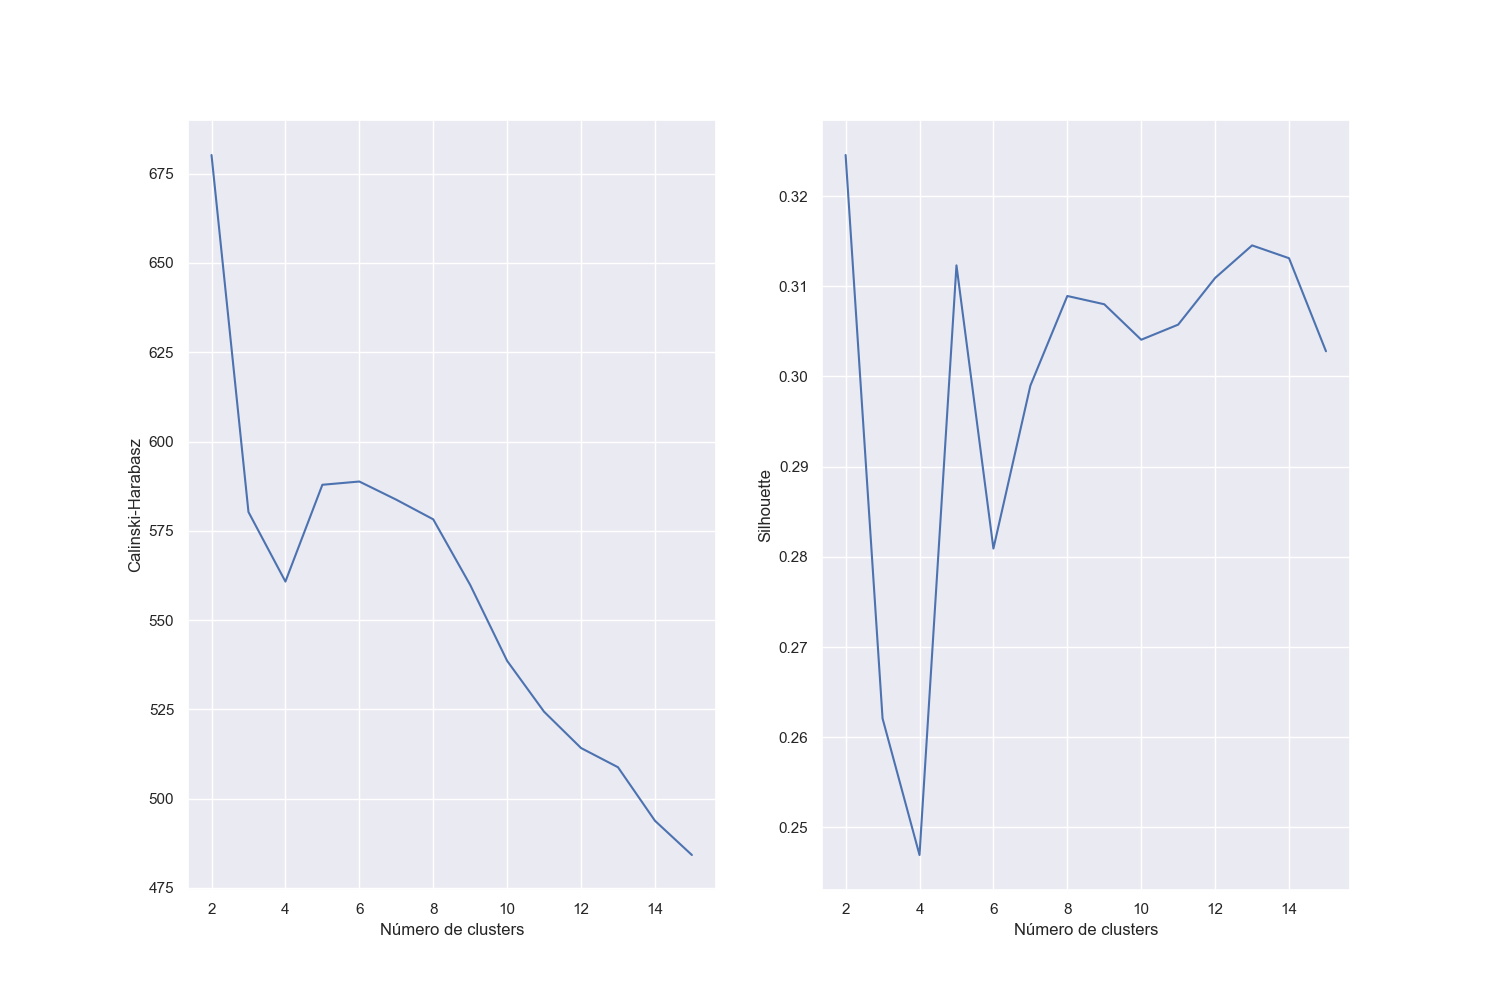
\includegraphics[width=1.2\textwidth, height=0.45\textheight]{./caso1/param_kmeans}
    \caption{Caso 1 - Comparación coeficientes según el número de clusters - KMeans}
    \label{fig:param_kmeans1}
\end{figure}

Para un número muy bajo de clusters, 2, ambos índices alcanzan sus valores máximos. Esto se debe a que al distinguir entre tan solo dos grupos es más fácil conseguir que los elementos queden cerca de su centro. Al ir aumentando el número de grupos, será más complicado diferenciar los elementos de la frontera, disminuyendo los coeficientes.

Observamos que ambos coeficientes alcanzan un máximo local en 5 clusters, por lo que nuestra estimación por defecto fue acertada.

El coeficiente Calinski-Harabasz disminuye a medida que aumenta el número de clusters, pues aunque estén más concentrados, las diferencias entre ellos serán menores. Este hecho afecta más a este coeficiente que al coeficiente Silhouette, que a pesar de sufrir un mínimo local para 6 grupos, aumenta y se mantiene en el rango $[0.30, 0.32]$ a partir de 8 clusters.

\subsection{Birch}


\subsection{Interpretación de la segmentación}
% Conclusiones generales

\section{Caso de estudio 2 - Sin deseo de tener hijos}

Para el segundo caso de estudio, decidimos analizar el conjunto formado por las \textit{mujeres que no desean tener hijos}. Así, nos quedamos con las mujeres que respondieron no a la pregunta ``¿Le hubiera gustado o le gustaría tener hijos?'', esto es, contiene un 6 en la columna \texttt{DESEOHIJOS}. El subconjunto elegido está formado por 1806 objetos que deseamos agrupar para obtener más información.

Podemos observar el histograma de la variable \texttt{M\_NOHIJOS1} en la Figura \ref{fig:m_nohijos}. Esta variable contiene el primer motivo por el que la mujer en cuestión no ha tenido hijos.

\begin{figure}[H]
    \centering
    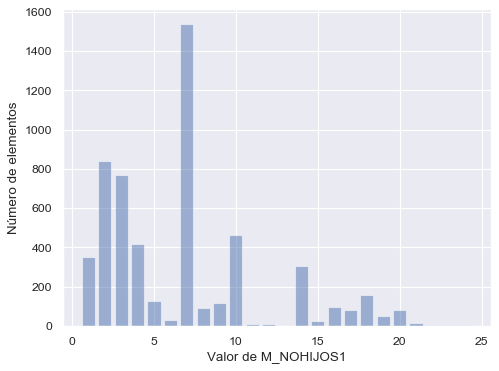
\includegraphics[width=0.75\textwidth]{./caso2/M_NOHIJOS1_tam}
    \caption{Caso 2 - Opción elegida en la encuesta en la pregunta ``Primer motivo por el que no ha tenido hijos''}
    \label{fig:m_nohijos}
\end{figure}

A continuación se lista el significado de cada una de estas opciones:

\begin{enumerate}
\addtocounter{enumi}{-1}
\item No me quedaba embarazada o no conseguí llevar un embarazo a término.
\item No he tenido una pareja o ésta no era adecuada.
\item No quiero ser madre o aún no quiero.
\item Deseaba seguir estudiando.
\item Problemas o molestias de salud.
\item Los embarazos, partos y cuidado de los hijos son duros para la mujer.
\item Demasiado joven para tener hijos.
\item Demasiada edad para tener hijos.
\item Entraría en conflicto con mi carrera profesional.
\item Insuficiencia de recursos económicos.
\item Malas condiciones de la vivienda.
\item Exceso de trabajo en el hogar.
\item Carencia o carestía de escuelas infantiles.
\item Por la situación laboral (propia o de la pareja).
\item Temor a que el hijo/a nazca con problemas de salud.
\item Supone perder libertad y no tener tiempo para realizar otras  actividades.
\item Por las preocupaciones y problemas que entraña criar a los hijos.
\item Dificultad para conciliar la vida laboral y familiar .
\item Mi pareja no ha querido.
\item No me gusta el modelo de sociedad actual para un niño.
\item Otros motivos.
\item Cuidar de otros familiares.
\item No convivo con mi pareja.
\item No he tenido la oportunidad de formar una familia.
\end{enumerate}

Apoyándonos en los motivos fundamentales que llevan a las mujeres a no desear tener hijos elegiremos las variables utilizadas para el agrupamiento. La principal razón que lleva a las mujeres a no tener hijos es que piensan que son demasiado mayores para ello (motivo 7), seguido de que no quieran ser madre aún o desean seguir estudiando (motivos 2 y 3) y las malas condiciones en la vivienda (motivo 10). Por ello, las variables elegidas para realizar clustering son:

\begin{itemize}
\item \textbf{EDAD} en años de la mujer entrevistada.
\item \textbf{SATISFACEVI} representa el grado de satisfacción con la vivienda. Es una escala del 0 al 10, donde 10 significa completamente satisfecho y 5 medianamente satisfecho.
\item \textbf{EDADIDEAL} es la edad que la entrevistada considera más adecuada para tener el primer hijo.
\item \textbf{ESTUDIOSA} simboliza el nivel de estudios alcanzados. Es una variable categórica que se representa con valores del 1 al 9, donde 1 denota menos que primaria, 5 educación postsecundaria no superior, 7 y 8 grados universitarios y 9 enseñanzas de doctorado.
\end{itemize}

El código necesario para ejecutar los diferentes algoritmos filtrando el conjunto inicial al de las mujeres que no desean tener hijos y agrupando a partir de las variables anteriores se encuentra en el archivo \texttt{caso2.py}. Tras ejecutarlo obtenemos los resultados recogidos en la Tabla \ref{tab:algorithms2}.

\begin{table}[H]
\centering
\caption{Resultados caso de estudio 2}
\label{tab:algorithms2}
\begin{tabular}{lrrrr}
\toprule
Algoritmo & Tiempo ($s$) & Calinski-Harabasz & Silhouette & Número de clusters\\
\midrule
KMeans & 0.139 & 920.360 & 0.29447 & 5 \\
MeanShift & 19.005 & 56.152 & 0.32798 & 2 \\
Birch & 0.119 & 522.766 & 0.32363 & 5 \\
DBSCAN & 0.037 & 19.834 & 0.26498 & 3 \\
Ward & 0.133 & 743.780 & 0.22985 & 5 \\
\bottomrule
\end{tabular}
\end{table}

En cuanto a tiempos de ejecución vuelve a destacar el elevado valor que alcanza MeanShift en comparación al resto de algoritmos, los motivos son los explicados en la Sección \ref{sec:caso1}.

Atendiendo al número de clusters, observamos que los algoritmos en los que no fijamos este valor crean un número muy bajo de clusters. De hecho, atendiendo a la salida del programa comprobamos que en ambos casos están realizando un único cluster con el 98\% de los valores. Concluimos que necesitamos adecuar los parámetros de estos algoritmos para que se ajusten al conjunto de datos y puedan generar algún tipo de segmentación.

Destaca también en la Tabla \ref{tab:algorithms2} que el índice Silhouette del algoritmo Birch supera al de KMeans y Ward, mientras que su índice Calinski-Harabasz es inferior al de los otros dos. Esto se debe a que de los 5 grupos creados por Birch, dos de ellos son muy pequeños y se ajustan muy bien a los datos que recogen, aunque la distancia entre los elementos del cluster sea baja. Que los clusters no estén muy poblados perjudica al coeficiente Calinski-Harabasz. El algoritmo que obtiene mayor valor para este coeficiente es KMeans.

A raíz de estas conclusiones iniciales decidimos estudiar el algoritmo KMeans y DBSCAN en el que trataremos de realizar un ajuste de parámetros con el que obtenga un desempeño adecuado.

\subsection{Análisis KMeans}

Comenzamos estudiando la segmentación obtenida tras aplicar el algoritmo KMeans. En primer lugar, vemos en la Figura \ref{fig:KMeans_tam2} que el reparto entre los grupos está igualado, excepto para el cluster 0, cuyo tamaño es aproximadamente la mitad que el resto.

\begin{figure}[H]
    \centering
    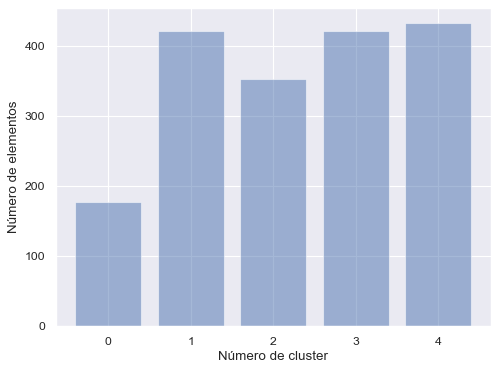
\includegraphics[width=0.6\textwidth]{./caso2/KMeans_tam_clusters}
    \caption{Caso 2 - Tamaño de cluster - KMeans}
    \label{fig:KMeans_tam2}
\end{figure}

Para hacernos una idea de cómo ha sido el reparto y qué importancia ha tenido cada variable para determinar los grupos, atendemos a la matriz de dispersión, la podemos encontrar en la Figura \ref{fig:KMeans_scattermatrix2}. Las variables EDAD Y ESTUDIOSA nos permiten separar 4 de estos grupos, el quinto se ve separado de los por su valor de SATISFACEVI.

\begin{figure}[H]
    \centering
    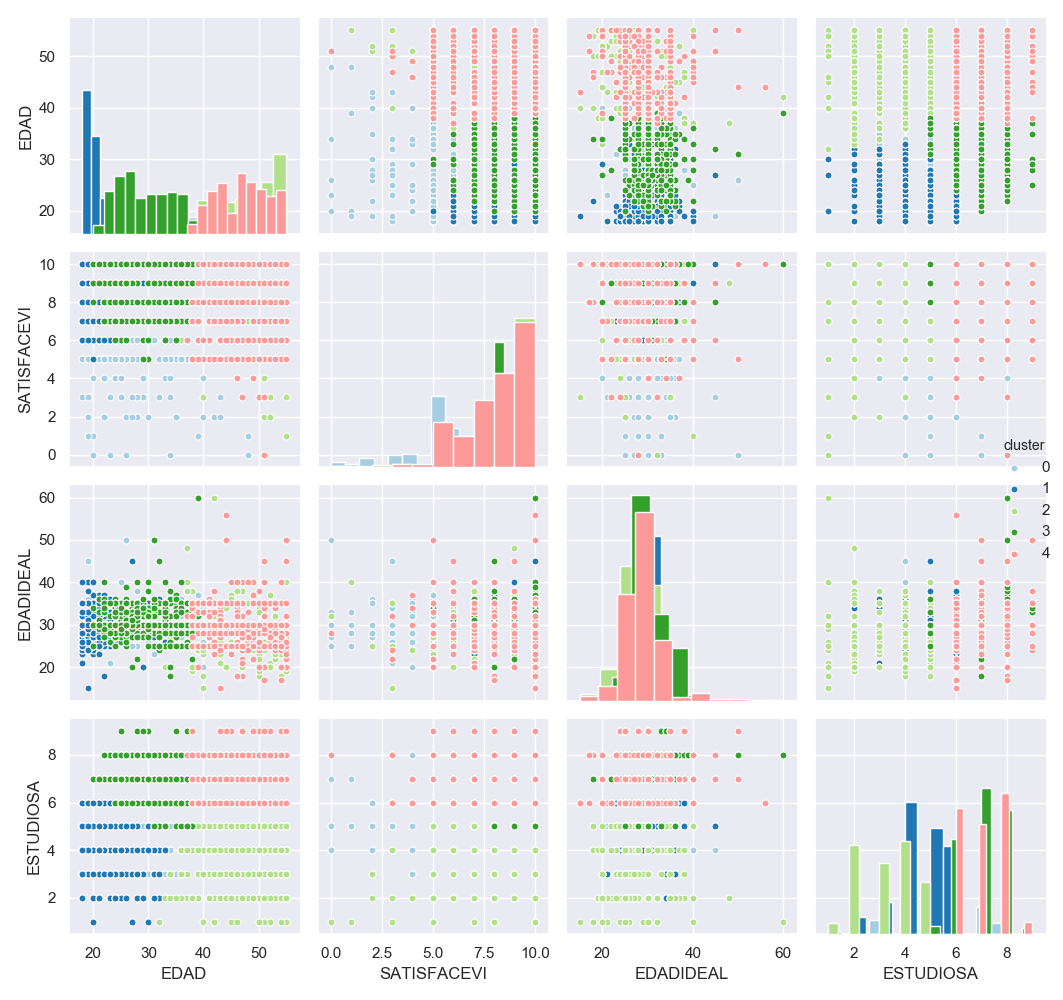
\includegraphics[width=1\textwidth]{./caso2/KMeans_scattermatrix}
    \caption{Caso 2 - Matriz de dispersión - KMeans}
    \label{fig:KMeans_scattermatrix2}
\end{figure}

Para examinar cuáles son las características que determinan la pertenencia a cada grupo, además de a la matriz de dispersión, atenderemos al mapa de calor de las variables que encontramos en la Figura \ref{fig:KMeans_heatmap2}. Sabemos que los clusters son convexos, luego, asumiendo concentración, la información obtenida de este gráfico será significativa.

\begin{figure}[H]
    \centering
    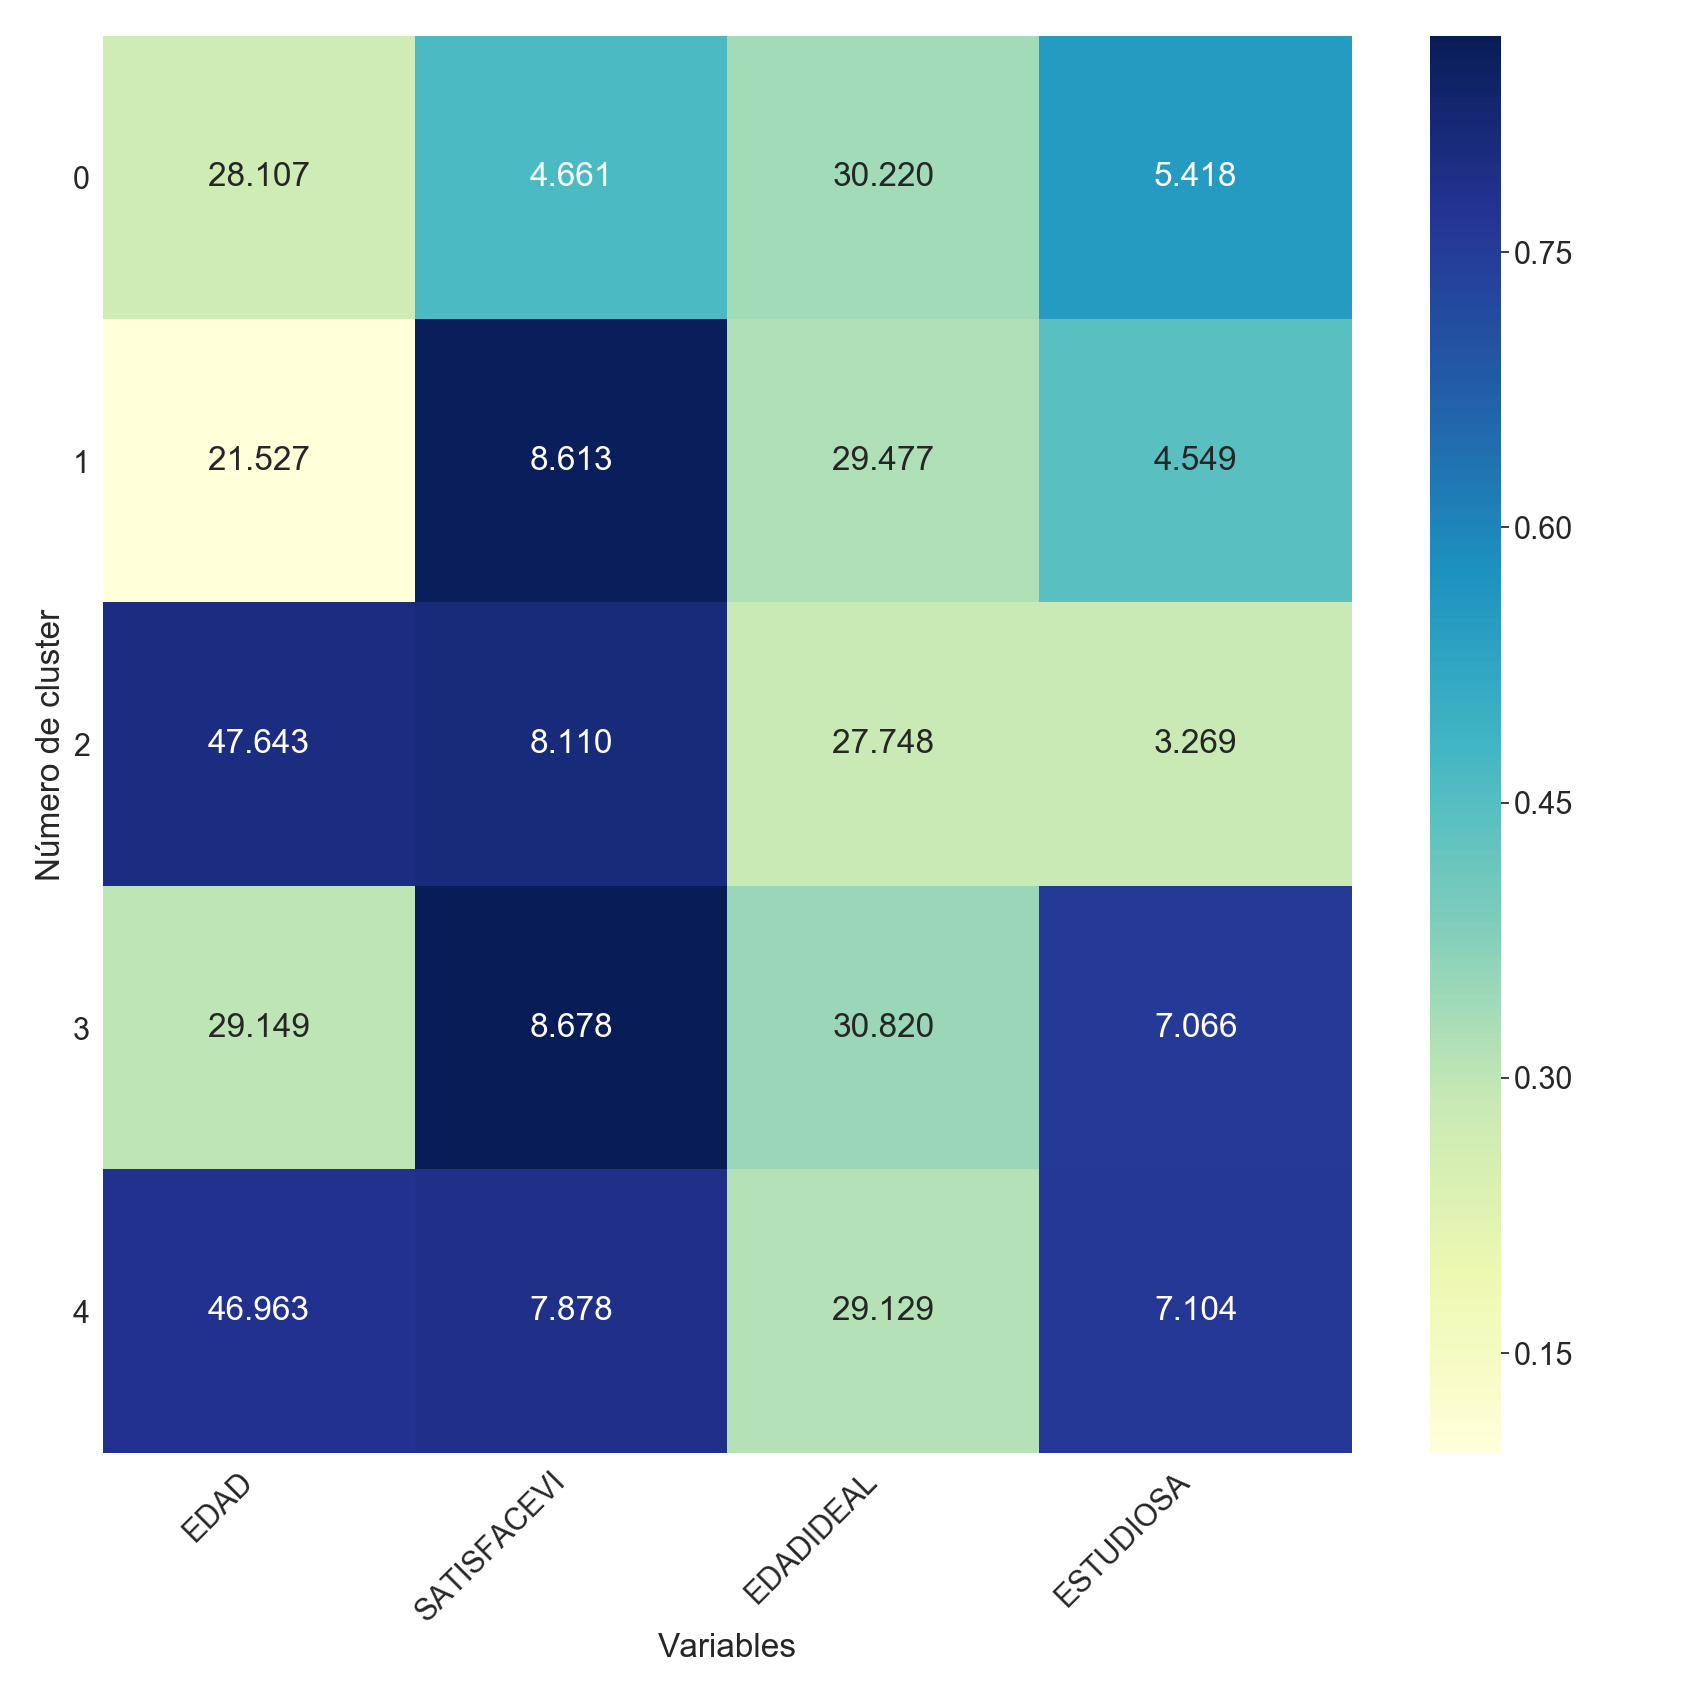
\includegraphics[width=1\textwidth]{./caso2/KMeans_heatmap}
    \caption{Caso 2 - Mapa de calor - KMeans}
    \label{fig:KMeans_heatmap2}
\end{figure}

Rellenaremos una tabla con las propiedades de cada grupo, sabiendo qué tipo de valores toma para cada variable, podremos comprender mejor la naturaleza de los mismos. En la Tabla \ref{tab:KMeans_carac2} se recoge esta información, como el heatmap no nos da rangos, podemos establecerlos a partir de este valor. Por ejemplo, diremos que la edad baja será la que ronde los 20 años (menor que 25), media entre 25 y 35 y alta más de 35. El grado de satisfacción con la vivienda lo consideraremos bajo cuando sea menor que 5 y alto cuando sea mayor que 5. La edad ideal para tener el primer hijo se dirá baja cuando sea menor que 28 años, media cuando esté entre 28 y 35 y alta cuando supere los 35 años. 

% Tabla características de los grupos generados por KMeans
\begin{table}[H]
\centering
\caption{Caso 2 - Características de los grupos - KMeans}
\label{tab:KMeans_carac2}
\begin{tabular}{lrrrr}
\toprule
Cluster & EDAD & SATISFACEVI & EDADIDEAL & ESTUDIOSA\\
\midrule
0 & Media & Bajo & Media & Educación postsecundaria \\
1 & Baja & Alto & Media & Educación secundaria \\
2 & Alta & Alto & Baja & Primera etapa de educación secundaria \\
3 & Media & Alto & Media & Grado universitario \\
4 & Alta & Alto & Media & Grado universitario \\
\bottomrule
\end{tabular}
\end{table}

Hay valores que son similares para cuatro de los grupos excepto uno, estos son determinantes para distinguir a dicho grupo de los demás. El grado de satisfacción con la vivienda es en general alto, excepto en el cluster 0, formado por mujeres a las que no satisface su vivienda. Notamos que este era el cluster de menor tamaño. Por otro lado, la edad considerada ideal para tener el primer hijo, aunque ronde valores similares, es significativamente más baja en el cluster 2. Las mujeres de este grupo se quedaron en la educación secundaria, es posible que el no dar importancia a los estudios y la edad a la que finalizarían los mismos sea el motivo fundamental para que baje esta edad ideal.

Los clusters 3 y 4 son parecidos, agrupan a mujeres con un grado universitario, para diferenciarlos atendemos a la variable edad, que en el caso del cluster 3 será menor que 35 años y en el 4 mayor. Por último, el cluster 1 es el que une a las mujeres más jóvenes, que han estudiado la educación secundaria.

\subsubsection{Análisis de parámetros}

Aunque los grupos obtenidos son, aparentemente, significativos, podemos comprobar qué habría ocurrido si en lugar de en 5 grupos hubiéramos realizado una segmentación en menos y más valores y ver cómo esto habría afectado a los coeficientes.

Para variar las opciones de este parámetro se utiliza el \textit{script} \texttt{caso2-kmeans.py}, en el que el parámetro \texttt{n\_clusters} se mueve en el rango de enteros $[2,15]$. En la Tabla \ref{tab:param_kmeans2} vemos los resultados obtenidos para los distintos valores del parámetro.

% Tablas comparativas para el análisis de parámetros
\begin{table}[H]
\centering
\caption{Resultados cambio de parámetros KMeans}
\label{tab:param_kmeans2}
\begin{tabular}{lrrrr}
\toprule
Número de clusters & Tiempo ($s$) & Calinski-Harabasz & Silhouette &\\
\midrule
2 & 0.262 & 1282.168 & 0.37326 \\
3 & 0.024 & 1106.125 & 0.35204 \\
4 & 0.056 & 996.314 & 0.28637 \\
5 & 0.079 & 921.725 & 0.29347 \\
6 & 0.117 & 852.970 & 0.27377 \\
7 & 0.125 & 809.926 & 0.26623 \\
8 & 0.145 & 784.366 & 0.26365 \\
9 & 0.203 & 755.025 & 0.25821 \\
10 & 0.194 & 724.466 & 0.24667 \\
11 & 0.262 & 692.991 & 0.24599 \\
12 & 0.365 & 670.809 & 0.23216 \\
13 & 0.543 & 643.188 & 0.22928 \\
14 & 0.374 & 629.141 & 0.23531 \\
15 & 0.440 & 612.722 & 0.22976 \\
\bottomrule
\end{tabular}
\end{table}

Destaca que el tiempo de ejecución no es creciente con el valor del parámetro, como lo fue en el caso de estudio 1. Para solo 2 clusters el algoritmo tarda lo mismo en ejecutarse que para crear 11 clusters. Para comparar el desempeño observaremos en la Figura  \ref{fig:param_kmeans2} como variaron los coeficientes Calinski-Harabaz y Silhouette al cambiar el número de clusters.

\begin{figure}[H]
    \centering
    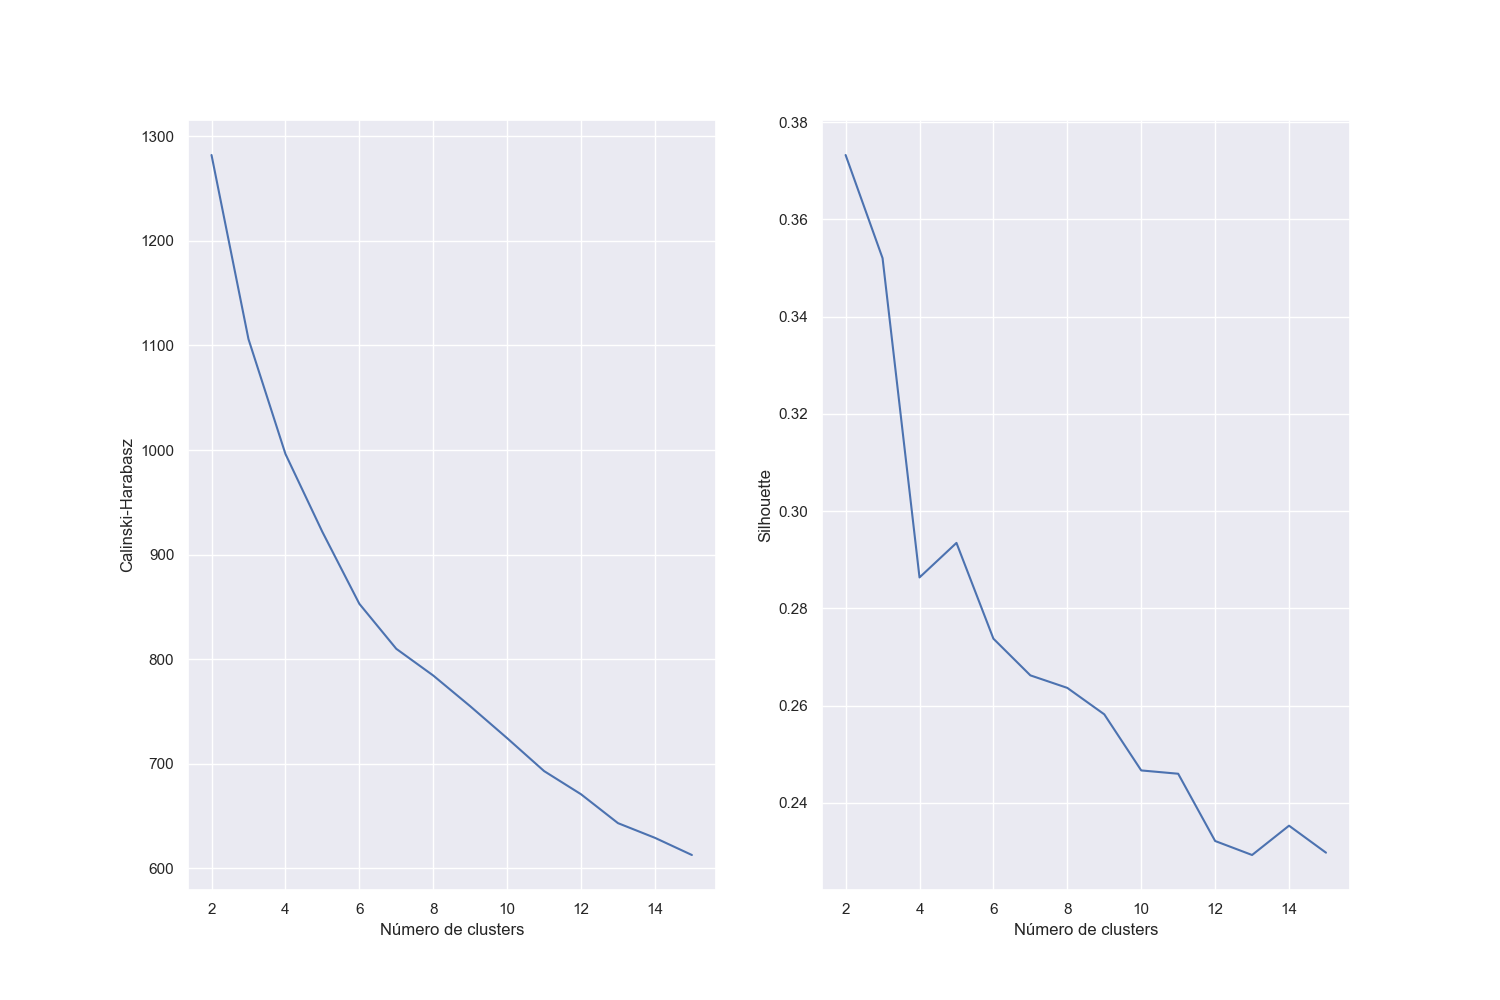
\includegraphics[width=1.2\textwidth, height=0.45\textheight]{./caso2/param_kmeans}
    \caption{Caso 2 - Comparación coeficientes según el número de clusters - KMeans}
    \label{fig:param_kmeans2}
\end{figure}

En esta ocasión la tendencia es similar para ambos coeficientes. A menor número de cluster, mayor valor del coeficiente y mejor agrupamiento. Podemos concluir que podemos dividir a las mujeres que no desean tener hijos en tan solo dos grupos para hacer una buena separación del conjunto. A medida que aumentemos el número de grupos a crear, las diferencias entre ellos no son lo suficientemente grandes y forzar esta división artificial en los grupos perjudica a los coeficientes consultados.

\subsection{Análisis DBSCAN}
\subsubsection{Análisis de parámetros}
En este caso, comenzamos con un análisis de parámetros, buscando aquel valor del radio que se adapte mejor al conjunto a estudiar. Para ello se ha implementado el \textit{script} \texttt{caso2-dbscan.py}, donde se prueba este algoritmo para diferentes valores del parámetro \texttt{eps} y \texttt{min\_samples}. En la Tabla \ref{tab:param_dbscan2} podemos observar los valores de los índices obtenidos para las distintas combinaciones de estos valores.

\begin{table}[H]
\centering
\caption{Resultados cambio de parámetros DBSCAN}
\label{tab:param_dbscan2}
\begin{tabular}{llrrrrr}
\toprule
$\varepsilon$ & min\_samples & Tiempo ($s$) & Calinski-Harabasz & Silhouette & Nº de clusters & Tam. $1^{er}$ cluster\\
\midrule
0.10 & 5 & 0.018 & 45.981 & -0.17517 & 47 & 26.19\% \\
0.15 & 5 & 0.033 & 47.571 & 0.25514 & 2 & 95.68\% \\
0.20 & 5 & 0.033 & 19.834 & 0.26498 & 3 & 98.23\% \\
0.25 & 5 & 0.042 & 17.014 & 0.35890 & 2 & 99.17\% \\
0.30 & 5 & 0.050 & 8.448 & 0.39872 & 2 & 99.72\% \\
\\
0.10 & 10 & 0.016 & 58.114 & -0.18197 & 30 & 44.96\% \\
0.15 & 10 & 0.029 & 53.289 & 0.21496 & 2 & 93.13\% \\
0.20 & 10 & 0.044 & 44.728 & 0.31036 & 2 & 97.67\% \\
0.25 & 10 & 0.053 & 21.548 & 0.35057 & 2 & 98.95\% \\
0.30 & 10 & 0.062 & 11.614 & 0.41289 & 2 & 99.61\% \\
\\
0.10 & 15 & 0.017 & 59.806 & -0.24084 & 15 & 65.12\% \\
0.15 & 15 & 0.036 & 97.678 & 0.18985 & 2 & 88.82\% \\
0.20 & 15 & 0.043 & 47.849 & 0.29252 & 2 & 97.23\% \\
0.25 & 15 & 0.048 & 29.719 & 0.35252 & 2 & 98.73\% \\
0.30 & 15 & 0.051 & 13.665 & 0.40924 & 2 & 99.56\% \\
\\
0.10 & 20 & 0.018 & 51.446 & -0.24913 & 12 & 76.08\% \\
0.15 & 20 & 0.036 & 71.282 & 0.06423 & 3 & 84.27\% \\
0.20 & 20 & 0.033 & 51.880 & 0.28787 & 2 & 96.90\% \\
0.25 & 20 & 0.040 & 31.183 & 0.34573 & 2 & 98.62\% \\
0.30 & 20 & 0.050 & 13.665 & 0.40924 & 2 & 99.56\% \\
\bottomrule
\end{tabular}
\end{table}


Incluso conociendo el valor de ambos coeficientes para unos parámetros fijos, es complicado decidir qué valores de los mismos tomar.

Descartamos el valor $\varepsilon = 0.1$, pues para cualquier número de muestras mínimo consigue un coeficiente Silhouette negativo. Al ser tan pequeña la distancia que determina cuándo un objeto es densamente alcanzable a partir de otro, se pueden alcanzar menos objetos a partir de uno dado y por ello aumenta el número de clusters, hasta 47 en el peor caso, generando un agrupamiento incorrecto.

La tónica general es la misma para diferente número mínimo de muestras: al aumentar el valor $\varepsilon$ crece el coeficiente Silhouette y disminuye el coeficiente Calinski-Harabasz. Intentando conseguir una buena relación entre ambos coeficientes escojo como valores de los parámetros: \texttt{eps = 0.2, min\_samples = 10}.

Como DBSCAN suele agrupar los objetos que no corresponden a ningún grupo en particular en un único grupo, esto provoca que en el peor caso tengamos dos grupos: uno mayoritario y otro con los \textit{outliers}. Observamos que el valor $\varepsilon = 0.1$ es muy pequeño y genera demasiados grupos, pero $\varepsilon = 0.15$ es muy grande y en la mayoría de los casos genera tan solo dos grupos.

Como la información obtenida es insuficiente, volvemos a ejecutar el \textit{script}, ahora para algunos valores $\varepsilon$ en el rango $[0.1, 0.15]$. Los resultados obtenidos esta vez los podemos encontrar en la Tabla \ref{tab:param_dbscan22}.

\begin{table}[H]
\centering
\caption{Resultados cambio de parámetros DBSCAN, $\varepsilon \in [0.1, 0.15]$}
\label{tab:param_dbscan22}
\begin{tabular}{llrrrrr}
\toprule
$\varepsilon$ & min\_samples & Tiempo ($s$) & Calinski-Harabasz & Silhouette & Número de clusters & Tam. $1^{er}$ cluster\\
\midrule
0.10 & 5 & 0.018 & 45.981 & -0.17517 & 47 & 26.19\% \\
0.11 & 5 & 0.022 & 84.449 & -0.15446 & 19 & 19.71\% \\
0.12 & 5 & 0.022 & 94.623 & -0.13734 & 18 & 20.38\% \\
0.13 & 5 & 0.024 & 25.566 & 0.03605 & 3 & 92.41\% \\
0.14 & 5 & 0.028 & 46.138 & 0.24058 & 2 & 94.91\% \\
0.15 & 5 & 0.028 & 47.571 & 0.25514 & 2 & 95.68\% \\
\\
0.10 & 10 & 0.017 & 58.114 & -0.18197 & 30 & 44.96\% \\
0.11 & 10 & 0.022 & 83.977 & -0.17966 & 16 & 33.89\% \\
0.12 & 10 & 0.021 & 131.384 & -0.12640 & 11 & 25.08\% \\
0.13 & 10 & 0.024 & 48.759 & 0.04495 & 3 & 85.60\% \\
0.14 & 10 & 0.026 & 60.746 & 0.20641 & 2 & 91.92\% \\
0.15 & 10 & 0.026 & 53.289 & 0.21496 & 2 & 93.13\% \\
\\
0.10 & 15 & 0.017 & 59.806 & -0.24084 & 15 & 65.12\% \\
0.11 & 15 & 0.019 & 90.783 & -0.17799 & 16 & 45.07\% \\
0.12 & 15 & 0.022 & 123.793 & -0.13657 & 10 & 34.99\% \\
0.13 & 15 & 0.024 & 68.439 & -0.04772 & 3 & 79.01\% \\
0.14 & 15 & 0.032 & 64.467 & 0.05823 & 3 & 85.27\% \\
0.15 & 15 & 0.025 & 97.678 & 0.18985 & 2 & 88.82\% \\
\\
0.10 & 20 & 0.016 & 51.446 & -0.24913 & 12 & 76.08\% \\
0.11 & 20 & 0.030 & 90.455 & -0.16712 & 12 & 60.30\% \\
0.12 & 20 & 0.020 & 110.723 & -0.20185 & 12 & 46.23\% \\
0.13 & 20 & 0.023 & 237.450 & 0.16647 & 2 & 69.27\% \\
0.14 & 20 & 0.033 & 151.269 & 0.16536 & 2 & 80.40\% \\
0.15 & 20 & 0.029 & 71.282 & 0.06423 & 3 & 84.27\% \\
\bottomrule
\end{tabular}
\end{table}

En este caso obtenemos incluso peores resultados, aparecen más casos con coeficiente Silhouette negativo, buscamos acercarnos a esa combinación $\varepsilon$, \texttt{min\_samples} que proporcione un coeficiente Silhouette positivo y unos clusters de tamaño más equilibrado. Seguimos haciendo pruebas (que no se incluyen por falta de interés) hasta decidir que los valores de los parámetros a tomar serán \texttt{eps = 0.128, min\_samples = 20}.

Sin embargo, aunque los resultados pudieran parecer más esperanzadores, pues para estos parámetros se crean 4 clusters diferentes y el primero de ellos contiene al 60\% del conjunto, de los otros tres hay dos que contienen el 2 y 3 \% del conjunto, mientras que el que contiene al 36 \% es el cluster -1 que agrupa a los elementos que no se ajustan a ningún grupo.

Concluimos que DBSCAN no se ajusta a este conjunto de datos. Además, para afinar la búsqueda de parámetros sería necesario algún otro tipo de algoritmo que de forma automática probara con una cantidad suficiente de opciones para conseguir los mejores resultados.

\subsection{Birch}
Para que el análisis de este caso de estudio no quede incompleto, tras las dificultades con DBSCAN, se decide analizar los resultados aportados por el algoritmo Birch. Ya habíamos notado que los grupos generados son desiguales, en la Figura \ref{fig:birch_tam2} observamos como, aunque nos devuelva 5 clusters, en la práctica solo se han realizado 3 grupos: los correspondientes a los clusters 1, 2 y 4.

\begin{figure}[H]
    \centering
    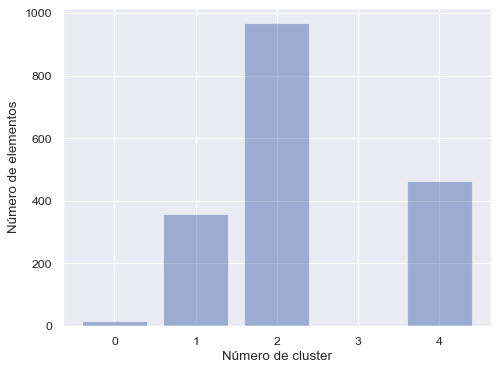
\includegraphics[width=0.5\textwidth]{./caso2/Birch_tam_clusters}
    \caption{Caso 2 - Tamaño de cada cluster - Birch}
    \label{fig:birch_tam2}
\end{figure}

Comenzamos, como en el resto de casos, observando la matriz de dispersión, que encontramos en la Figura \ref{fig:birch_scattermatrix2}. En ella los grupos que destacan son los que ya habíamos señalado el 1, 2 y 4. En una primera observación destacamos que se ven distinguidos por la variable EDAD y EDADESTUDIOSA. 

\begin{figure}[H]
    \centering
    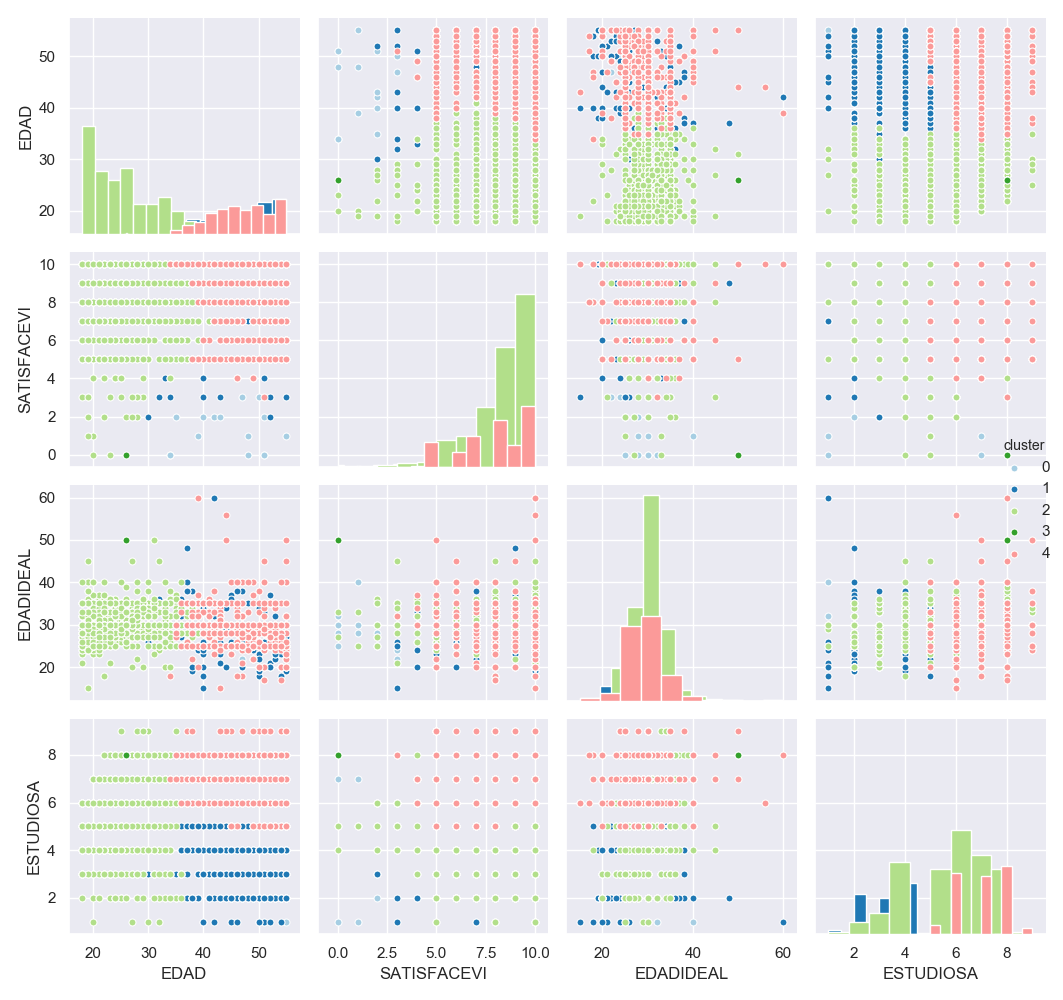
\includegraphics[width=1\textwidth]{./caso2/Birch_scattermatrix}
    \caption{Caso 2 - Matriz de dispersión - Birch}
    \label{fig:birch_scattermatrix2}
\end{figure}

Para determinar las características de los grupos nos apoyamos en un histograma\footnote{Nos decantamos por un histograma en vez de una función de distribución porque varias de las variables son discretas. A pesar de todo se incluye una línea que muestra la distribución seguida.}, encontrado en la Figura \ref{fig:birch_dist2}, que nos permitirá crear la tabla de características.

\begin{figure}[H]
    \centering
    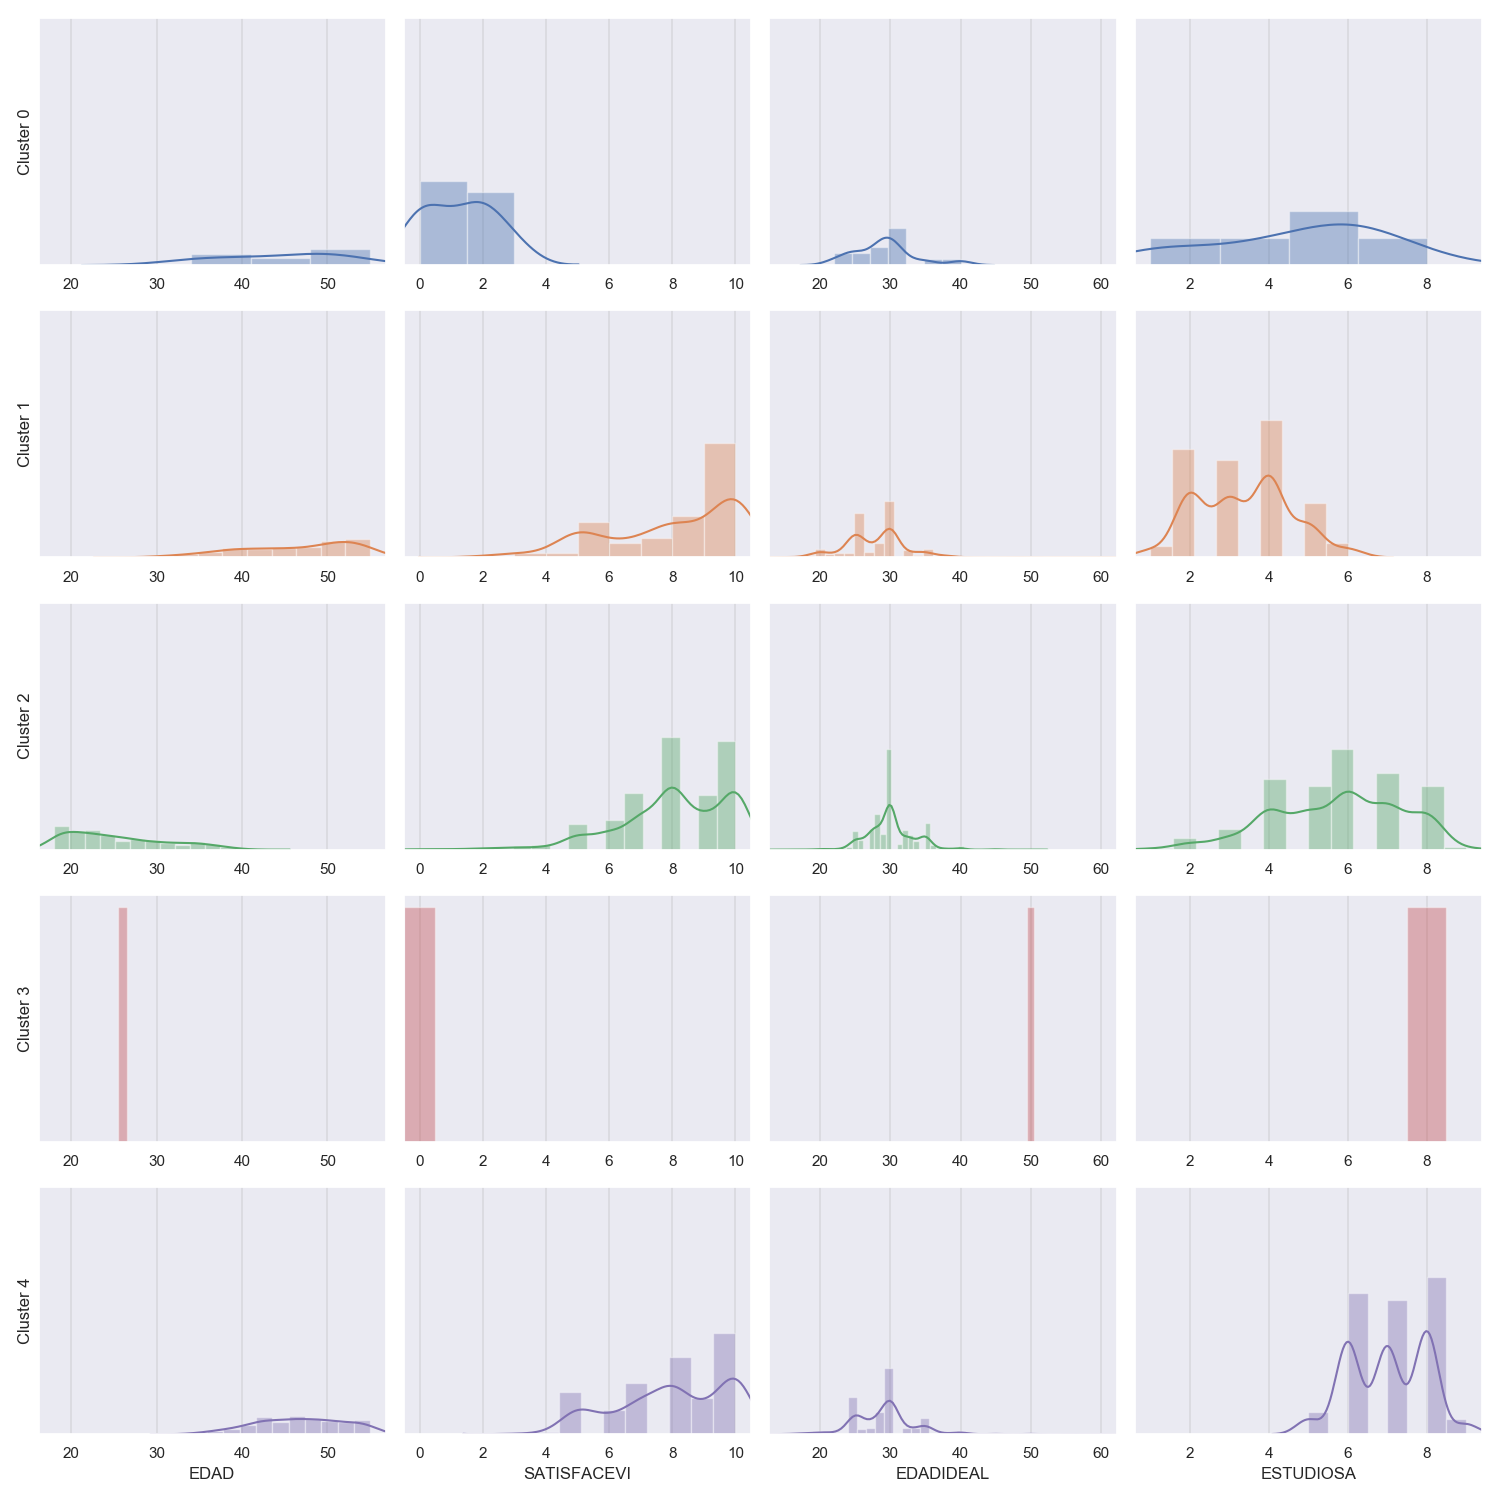
\includegraphics[width=1\textwidth]{./caso2/Birch_distplot}
    \caption{Caso 2 - Histograma - Birch}
    \label{fig:birch_dist2}
\end{figure}

En el histograma destaca que el cluster 3, que contenía muy pocos elementos, se ajusta perfectamente a ellos, es una barra vertical que en un mismo valor representa a todos los elementos del cluster. Sin embargo, no estamos interesados en estos valores.

En la Tabla \ref{tab:birch_carac2} encontramos las características de los grupos, agrupando los valores de las variables igual que se hizo en el caso del algoritmo KMeans.

% Tabla características de los grupos generados por KMeans
\begin{table}[H]
\centering
\caption{Caso 2 - Características de los grupos - KMeans}
\label{tab:birch_carac2}
\begin{tabular}{lrrrr}
\toprule
Cluster & EDAD & SATISFACEVI & EDADIDEAL & ESTUDIOSA\\
\midrule
1 & Alta & Alto & Media-baja & Hasta educación secundaria \\
2 & Media - baja & Media & Baja & Educación secundaria - Grado universitario \\
4 & Alta & Alto & Media-baja & Formación profesional - Grado universitario \\
\bottomrule
\end{tabular}
\end{table}

Así, podemos distinguir los grupos 1 y 4 por el nivel de estudios de las mujeres que pertenecen a ellos, ambos están formados por mujeres mayores de 35 que están satisfechas con su vivienda y consideran que la edad apropiada para tener el primer hijo es menor a 30 años. El grupo restante tiene un grado de agrado con su vivienda medio, las mujeres son más jóvenes y los niveles de estudio son diferentes en todas ellas, teniendo menor importancia para determinarlo.

\subsection{Interpretación de la segmentación}
% Conclusiones generales
En general, considero que ha sido una mala idea elegir tantas variables discretas cuando los algoritmos elegidos se basan en distancias. Los resultados de los algoritmos no han sido demasiado buenos en ningún caso. Además, destaca el esfuerzo empleado en tratar de ajustar DBSCAN y MeanShift (aunque no se incluya, se realizó un análisis similar al realizado con DBSCAN sin obtener ningún progreso).

En cuanto los clusters obtenidos en los algoritmos estudiados, aunque los dos algoritmos no generen los mismos grupos, sí que los diferencian a partir de las variables estudiadas, teniendo más peso el nivel de estudios en el caso del algoritmo Birch.
\newpage
%%%%%%%%%%%%%%%%%%%%%%%%%%%%%%%%%%%%%%%%%%%%%%%%%%%%%%%%%%%%%%%%%%%
%       REFERENCIAS
%%%%%%%%%%%%%%%%%%%%%%%%%%%%%%%%%%%%%%%%%%%%%%%%%%%%%%%%%%%%%%%%%%%
\printbibliography

%datos
%http://scikit-learn.org/stable/modules/clustering.html
%https://pythonspot.com/matplotlib-bar-chart/ -> Gráficos de tamaño de cluster
% https://matplotlib.org/3.1.1/tutorials/introductory/lifecycle.html -> same
% https://matplotlib.org/gallery/images_contours_and_fields/image_annotated_heatmap.html#sphx-glr-gallery-images-contours-and-fields-image-annotated-heatmap-py -> heatmap
%https://docs.w3cub.com/scikit_learn/auto_examples/cluster/plot_birch_vs_minibatchkmeans/ -> centros birch
\end{document}
